% Laporan akhir penelitian: pengaruh konstanta kosmologi pada sudut pembelokan cahaya di ruang-waktu Kerr-de Sitter.
% Kompilasi (dari folder ini):  tectonic laporan_akhir.tex
%   atau: pdflatex laporan_akhir && bibtex laporan_akhir && pdflatex laporan_akhir && pdflatex laporan_akhir
% Data, gambar, dan tabel dibuat oleh generate_results.py.
\documentclass[11pt,a4paper]{article}

\usepackage{iftex}
\ifPDFTeX
  \usepackage[T1]{fontenc}
  \usepackage[utf8]{inputenc}
  \usepackage{lmodern}
\fi
\usepackage[indonesian]{babel}
\usepackage[a4paper,margin=2.5cm]{geometry}
\usepackage{amsmath,amssymb}
\usepackage{icomma}
\usepackage{graphicx}
\usepackage{booktabs}
\usepackage{array}
\usepackage[font=small,labelfont=bf]{caption}
\usepackage{tikz}
\usetikzlibrary{angles,quotes,calc,babel}
\usepackage[section]{placeins}
\usepackage[round,authoryear]{natbib}
\usepackage[hidelinks]{hyperref}

\addto\captionsindonesian{%
  \renewcommand{\refname}{Daftar Pustaka}%
  \renewcommand{\contentsname}{Daftar Isi}%
  \renewcommand{\figurename}{Gambar}%
  \renewcommand{\tablename}{Tabel}%
  \renewcommand{\abstractname}{Abstrak}%
}

\newcommand{\dd}{\mathrm{d}}
\setlength{\parskip}{0.4em}

% Isi tabel dibuat oleh generate_results.py; dibaca dengan \input primitif agar aman di dalam tabular
\makeatletter
\newcommand{\isitabel}[1]{\@@input #1 }
\makeatother

\title{\textbf{Laporan Akhir Penelitian}\\[6pt]
  \Large Pengaruh Konstanta Kosmologi pada Sudut Pembelokan Cahaya\\
  di Sekitar Lubang Hitam Kerr--de Sitter:\\
  Simulasi Numerik dan Perbandingan dengan Hasil Analitik}
\author{Nugie Saputra\\[2pt]
  \small Program Studi Fisika, FMIPA Universitas Tanjungpura}
\date{November 2026}

\begin{document}
\maketitle

\begin{abstract}
\noindent
Sudut pembelokan cahaya di bidang ekuator ruang-waktu Kerr--de Sitter dihitung secara numerik untuk
11 nilai spin ($-0{,}99 \le a \le 0{,}99$) dan 13 nilai konstanta kosmologi
($-5\times10^{-6} \le \Lambda \le 5\times10^{-6}$, satuan $M^{-2}$) pada parameter dampak $b = 7M$.
Persamaan gerak foton diturunkan dari Hamiltonian $H = \tfrac12 g^{\mu\nu}p_\mu p_\nu$ secara simbolik
dan diintegrasikan dengan metode Runge--Kutta orde empat. Sudut defleksi didefinisikan pada jarak hingga
seperti pada artikel acuan \citep{ishihara2016gravitational,belhaj2022light,huang2025influence}, yaitu
$\delta = \Psi_O - \Psi_S + \phi_{OS}$, dengan $\Psi$ sudut sinar yang diukur pengamat statis di posisi
sumber dan pengamat. Simulasi sesuai dengan solusi eksak (kuadratur integral pertama geodesik) hingga
$5{,}5\times10^{-7}{}^\circ$, dengan konservasi Hamiltonian $|H| \lesssim 5\times10^{-11}$. Hasil utamanya:
(i) spin prograde memperkecil dan spin retrograde memperbesar sudut defleksi, sesuai
\citet{congdon2022asymmetric}; (ii) konstanta kosmologi positif \emph{memperkecil} sudut defleksi dan
konstanta kosmologi negatif memperbesarnya, sesuai \citet{rindler2007contribution},
\citet{belhaj2022light}, dan \citet{huang2025influence}; besar perubahannya cocok dengan rumus analitik
Huang dkk.\ dan Belhaj dkk.\ dengan selisih di bawah $10\%$ pada $\Lambda = 10^{-6}$; (iii) efek pengurangan oleh
$\Lambda$ melemah untuk spin prograde, sesuai suku $a\Lambda$ dalam rumus analitik; dan (iv) pada spin
retrograde ekstrem $a = -0{,}99$, foton berada sangat dekat dengan orbit kritisnya sehingga pergeseran
parameter dampak kritis oleh $\Lambda$ membalik tren tersebut. Laporan ini juga menjelaskan mengapa
definisi berbasis sudut koordinat yang dipakai pada versi awal penelitian memberi tren $\Lambda$ yang
berlawanan.

\medskip\noindent
\textbf{Kata kunci:} pembelokan cahaya, lubang hitam Kerr--de Sitter, konstanta kosmologi, mekanika
Hamiltonian, Runge--Kutta orde empat
\end{abstract}

\tableofcontents
\newpage

% =====================================================================================
\section{Pendahuluan}

\subsection{Latar belakang}

Pembelokan cahaya oleh medan gravitasi merupakan salah satu prediksi klasik relativitas umum dan menjadi
dasar pelensaan gravitasi. Lubang hitam yang berotasi dideskripsikan oleh solusi Kerr
\citep{kerr1963gravitational,teukolsky2015kerr}. Rotasi menimbulkan efek \emph{frame dragging} yang membuat
foton prograde (searah rotasi) dan retrograde (berlawanan rotasi) dibelokkan secara berbeda
\citep{congdon2022asymmetric}. Konstanta kosmologi $\Lambda$, yang diperkenalkan Einstein pada 1917 dan
kini menjadi penjelasan paling sederhana bagi percepatan ekspansi alam semesta
\citep{ferrara2017einstein,cohen2018lambda}, mengubah struktur ruang-waktu di sekitar lubang hitam. Untuk
lubang hitam berotasi dengan $\Lambda > 0$, ruang-waktunya adalah Kerr--de Sitter, yang memiliki horizon
peristiwa sekaligus horizon kosmologis \citep{li2017entropy,ovalle2021kerr,hackmann2010geodesic}; kasus
tak berotasinya adalah Schwarzschild--de Sitter \citep{latief2023sifat}.

Apakah $\Lambda$ memengaruhi sudut pembelokan cahaya merupakan pertanyaan yang lama diperdebatkan.
Persamaan orbit foton di Schwarzschild--de Sitter, $\dd^2u/\dd\phi^2 + u = 3Mu^2$, tidak memuat $\Lambda$,
sehingga sempat disimpulkan bahwa $\Lambda$ tidak berpengaruh. \citet{rindler2007contribution}
menunjukkan bahwa kesimpulan itu keliru: sudut yang benar-benar terukur ditentukan juga oleh metrik, dan
$\Lambda > 0$ memperkecil sudut pembelokan. Pendekatan teorema Gauss--Bonnet pada jarak hingga
\citep{ishihara2016gravitational,arakida2018light} kemudian dipakai untuk lubang hitam berotasi
\citep{jusufi2018gravitational,jusufi2018deflection}, termasuk dengan konstanta kosmologi
\citep{belhaj2022light,huang2025influence,pantig2024testing}; semuanya memperoleh suku $\Lambda$ yang
memperkecil sudut defleksi. Di sisi lain, \citet{arakida2018light} menunjukkan bahwa suku orde $\Lambda$
lenyap bila sudut diukur relatif terhadap latar de Sitter, dan \citet{hu2022light} tidak menemukan efek
$\Lambda$ di luar jarak diameter sudut dalam model kosmologis Swiss-cheese. Pengaruh $\Lambda$ juga
tampak pada bayangan lubang hitam \citep{afrin2022estimating,pantig2024testing}. Jadi, besar dan tanda
pengaruh $\Lambda$ bergantung pada \emph{definisi} sudut defleksi yang dipakai.

Penelitian ini menghitung sudut defleksi secara numerik, tanpa pendekatan medan lemah, dan
membandingkannya dengan hasil analitik artikel-artikel tersebut. Hasil numerik
\citet{hasanuddin2012pembelokan} untuk ruang-waktu Kerr dipakai sebagai acuan validasi pada $\Lambda = 0$.

\subsection{Tujuan}

\begin{enumerate}
  \item Menurunkan persamaan gerak foton di ruang-waktu Kerr--de Sitter dari Hamiltonian secara simbolik
        dan menyelesaikannya secara numerik.
  \item Menghitung sudut defleksi untuk berbagai nilai spin $a$ dan konstanta kosmologi $\Lambda$ (positif
        dan negatif) dengan definisi yang sama seperti pada artikel acuan.
  \item Memvalidasi hasil numerik terhadap solusi eksak dan nilai literatur, serta membandingkannya dengan
        rumus analitik \citet{belhaj2022light} dan \citet{huang2025influence}.
  \item Menjelaskan mekanisme fisis pengaruh $a$ dan $\Lambda$ terhadap sudut defleksi.
\end{enumerate}

\subsection{Catatan tentang versi penelitian}

Pada versi awal penelitian (naskah skripsi), sudut defleksi dihitung sebagai selisih sudut azimut koordinat
$\lvert\Delta\phi - \pi\rvert$ antara titik awal dan titik akhir lintasan; versi kode tersebut tersimpan di
repositori penelitian dengan penanda \texttt{skripsi-v1.0}. Analisis kesesuaian dengan artikel acuan
menunjukkan bahwa besaran tersebut berbeda dari sudut defleksi yang didefinisikan pada artikel, dan memberi
tren $\Lambda$ dengan tanda berlawanan. Kode kemudian diperbaiki. Lintasan foton tidak berubah sama sekali, tetapi sudut defleksi utama kini mengikuti
definisi artikel (Subbab~\ref{subsec:definisi}). Seluruh data dalam laporan ini berasal dari kode yang
telah diperbaiki; perbandingan kedua definisi dibahas pada Subbab~\ref{subsec:dua-definisi}.

% =====================================================================================
\section{Landasan Teori}

\subsection{Metrik Kerr--de Sitter}

Dalam koordinat Boyer--Lindquist $(t, r, \theta, \phi)$ dan satuan geometris $G = c = 1$, metrik
Kerr--de Sitter yang dipakai dalam kode adalah
\begin{equation}
  \dd s^2 = -\frac{\Delta_r}{\Sigma}\left(\dd t - \frac{a\sin^2\theta}{\Xi}\,\dd\phi\right)^2
  + \frac{\Delta_\theta\sin^2\theta}{\Sigma}\left(a\,\dd t - \frac{r^2+a^2}{\Xi}\,\dd\phi\right)^2
  + \frac{\Sigma}{\Delta_r}\,\dd r^2 + \frac{\Sigma}{\Delta_\theta}\,\dd\theta^2,
  \label{eq:metrik}
\end{equation}
dengan
\begin{equation}
  \Sigma = r^2 + a^2\cos^2\theta,\quad
  \Delta_r = (r^2+a^2)\left(1 - \frac{\Lambda r^2}{3}\right) - 2Mr,\quad
  \Delta_\theta = 1 + \frac{\Lambda a^2\cos^2\theta}{3},\quad
  \Xi = 1 + \frac{\Lambda a^2}{3}.
\end{equation}
Bentuk ini identik dengan bentuk standar \citep{li2017entropy,hackmann2010geodesic} setelah penskalaan
waktu $t \to t/\Xi$. Untuk $\Lambda = 0$ metrik ini menjadi metrik Kerr, untuk $a = 0$ menjadi
Schwarzschild--de Sitter, dan $\Lambda < 0$ menghasilkan Kerr--anti-de Sitter. Akar-akar $\Delta_r = 0$
memberi horizon peristiwa $r_+$ dan, untuk $\Lambda > 0$, horizon kosmologis $r_c \approx \sqrt{3/\Lambda}$;
untuk $\Lambda = 5\times10^{-6}$ diperoleh $r_c \approx 773{,}6\,M$.

\subsection{Formulasi Hamiltonian dan persamaan orbit}

Geodesik null diperlakukan sebagai sistem Hamiltonian \citep{emam2021covariant,ritus2015lagrangian}
\begin{equation}
  H = \tfrac12\, g^{\mu\nu} p_\mu p_\nu = 0, \qquad
  \frac{\dd x^\mu}{\dd\tau} = \frac{\partial H}{\partial p_\mu}, \qquad
  \frac{\dd p_\mu}{\dd\tau} = -\frac{\partial H}{\partial x^\mu}.
  \label{eq:hamilton}
\end{equation}
Karena metrik tidak bergantung pada $t$ dan $\phi$, energi $E = -p_t$ dan momentum sudut $L = p_\phi$
kekal, dan parameter dampak didefinisikan sebagai $b = L/E$. Pada bidang ekuator, dengan $E = 1$,
$L = b$, $B = \Xi b$, dan $P = r^2 + a^2 - aB$, integral pertama geodesik memberi
\begin{equation}
  R(r) = P^2 - \Delta_r\,(B - a)^2, \qquad
  \frac{\dd\phi}{\dd r} = \frac{\Xi\left[a P/\Delta_r + (B - a)\right]}{\sqrt{R(r)}}.
  \label{eq:orbit}
\end{equation}
Titik balik (jarak terdekat) $r_\text{min}$ adalah akar terbesar $R(r) = 0$. Persamaan~\eqref{eq:orbit}
dipakai sebagai \emph{pembanding eksak}: sudut azimut $\phi_{OS}$ dihitung dengan kuadratur numerik
berpresisi tinggi, tanpa pendekatan medan lemah.

\subsection{Definisi sudut defleksi pada jarak hingga}
\label{subsec:definisi}

Ruang-waktu dengan $\Lambda \ne 0$ tidak datar asimtotik, sehingga sumber $S$ dan pengamat $O$ harus
berada pada jarak hingga ($r_+ < r < r_c$). \citet{ishihara2016gravitational} mendefinisikan sudut
defleksi pada jarak hingga sebagai
\begin{equation}
  \delta = \Psi_O - \Psi_S + \phi_{OS},
  \label{eq:definisi}
\end{equation}
dengan $\phi_{OS} = \phi_O - \phi_S$ sudut azimut yang ditempuh, serta $\Psi_S$ dan $\Psi_O$ sudut antara
sinar dan arah radial keluar di posisi sumber dan pengamat (Gambar~\ref{fig:skema}). Definisi ini dipakai
oleh \citet[Pers.~2.1]{belhaj2022light} dan \citet[Pers.~12]{huang2025influence}. Untuk ruang-waktu
berotasi, \citeauthor{huang2025influence} mengukur $\Psi$ dalam ruang optik Randers; bagian Riemann dari
metrik Randers konformal dengan metrik ruang pengamat statis (kecepatan-4 searah $\partial_t$), sehingga
$\Psi$ adalah sudut yang diukur pengamat statis. Dalam kerangka ortonormal pengamat tersebut,
\begin{equation}
  \tan\Psi = \frac{p_{\hat\phi}}{p_{\hat r}}, \qquad
  p_{\hat r} = \frac{p_r}{\sqrt{g_{rr}}}, \qquad
  p_{\hat\phi} = \frac{p_\phi - (g_{t\phi}/g_{tt})\,p_t}{\sqrt{g_{\phi\phi} - g_{t\phi}^2/g_{tt}}}.
  \label{eq:psi}
\end{equation}
Untuk Schwarzschild--de Sitter rumus ini menjadi $\sin\psi = b\sqrt{1 - 2M/r - \Lambda r^2/3}\,/\,r$,
dengan $\psi$ sudut lancip antara sinar dan garis radial. Di ruang datar $\delta = 0$ secara eksak, dan
untuk $\Lambda = 0$ dengan $r_S, r_O \to \infty$, $\delta$ menjadi sudut defleksi asimtotik yang biasa.

\begin{figure}[t]
  \centering
  \begin{tikzpicture}[scale=1.05, >=stealth]
    \coordinate (L) at (0,0);
    \coordinate (S) at (5,-0.8);
    \coordinate (O) at (-5,-0.8);
    \coordinate (C1) at (1.6,1.7);
    \coordinate (C2) at (-1.6,1.7);
    \coordinate (S2) at ($(L)!1.22!(S)$);
    \coordinate (O2) at ($(L)!1.22!(O)$);
    \coordinate (TS) at ($(S)!0.32!(C1)$);
    \coordinate (TO) at ($(O)!-0.32!(C2)$);
    \draw[gray] (L) -- (S2);
    \draw[gray] (L) -- (O2);
    \draw[very thick, ->] (S) .. controls (C1) and (C2) .. (O);
    \node at (0,1.55) {$\gamma$};
    \draw[->] (S) -- (TS);
    \draw[->] (O) -- (TO);
    \pic[draw, "$\Psi_S$", angle radius=0.55cm, angle eccentricity=1.6] {angle = S2--S--TS};
    \pic[draw, "$\Psi_O$", angle radius=0.75cm, angle eccentricity=1.45] {angle = O2--O--TO};
    \pic[draw, "$\phi_{OS}$", angle radius=0.45cm, angle eccentricity=1.7] {angle = S--L--O};
    \fill (L) circle (2.2pt) node[below=2pt] {$L$};
    \fill (S) circle (1.6pt) node[below right] {$S$};
    \fill (O) circle (1.6pt) node[below right] {$O$};
  \end{tikzpicture}
  \caption{Skema sudut defleksi pada jarak hingga (mengikuti \citealp{huang2025influence}). Cahaya
    bergerak dari sumber $S$ ke pengamat $O$ melewati lubang hitam $L$. $\Psi_S$ dan $\Psi_O$ adalah sudut
    antara sinar $\gamma$ dan arah radial keluar di $S$ dan $O$, sedangkan $\phi_{OS}$ adalah sudut azimut
    yang ditempuh.}
  \label{fig:skema}
\end{figure}

Dua besaran lain juga dihitung untuk perbandingan: nilai koordinat $\phi_{OS} - \pi$ dan nilai versi awal
penelitian $\lvert\phi_{OS} - \pi\rvert$. Nilai koordinat memuat \emph{offset} ruang datar
$-[\arcsin(b/r_S) + \arcsin(b/r_O)]$, kira-kira $-1{,}6^\circ$ untuk $b = 7M$ dan $r_S = 500M$.

\subsection{Hasil analitik pembanding}

\citet{rindler2007contribution} memperoleh sudut pembelokan satu sisi di Schwarzschild--de Sitter
\begin{equation}
  \psi_0 \approx \frac{2M}{R}\left(1 - \frac{2M^2}{R^2} - \frac{\Lambda R^4}{24M^2}\right),
\end{equation}
yang menunjukkan bahwa $\Lambda > 0$ memperkecil pembelokan. Untuk lubang hitam Kerr dengan konstanta
kosmologi, \citet[Pers.~5.1]{belhaj2022light} memperoleh dengan teorema Gauss--Bonnet
\begin{equation}
  \alpha \approx \frac{4M}{b} - \frac{4aM}{b^2} + \frac{b\Lambda M}{3}
  - \left(\frac{1}{u_R} + \frac{1}{u_S}\right)\frac{b\Lambda}{6}
  + \left(\frac{1}{u_R} + \frac{1}{u_S}\right)\frac{2a\Lambda}{3},
  \label{eq:belhaj}
\end{equation}
dengan $u = 1/r$. \citet[Pers.~24]{huang2025influence} memperoleh rumus yang lebih lengkap hingga orde
kedua dalam $M/b$, $a/b$, dan $\Lambda b^2$, yang suku-suku utamanya adalah
\begin{equation}
  \begin{split}
    \delta \approx{}& \frac{2M}{b}\sum_{i=O,S}\sqrt{1-b^2u_i^2}
    - \frac{\Lambda b}{6}\sum_{i=O,S}\frac{\sqrt{1-b^2u_i^2}}{u_i} \\
    & - \frac{2Ma}{b^2}\sum_{i=O,S}\sqrt{1-b^2u_i^2}
    + \frac{2a\Lambda}{3}\sum_{i=O,S}\frac{\sqrt{1-b^2u_i^2}}{u_i} + \dots
  \end{split}
  \label{eq:huang}
\end{equation}
ditambah suku-suku orde $M^2$, $M\Lambda$, dan $\Lambda^2$. Kedua rumus memuat tiga ciri utama: suku
$\mp 4aM/b^2$ (spin prograde memperkecil defleksi, sesuai \citealp{jusufi2018gravitational}), suku
$-\Lambda b\,r/6$ per sisi (konstanta kosmologi positif memperkecil defleksi), dan suku $+2a\Lambda r/3$
per sisi yang melemahkan efek $\Lambda$ untuk foton prograde. \citet[\S\,4.1.2]{huang2025influence} juga
mencatat bahwa bila yang dihitung hanya sudut azimut $\phi_{OS}$, suku $\Lambda$-nya justru positif,
$+\tfrac{\Lambda b^3}{6}\sum_i u_i/\sqrt{1-b^2u_i^2}$; hal ini dibahas pada
Subbab~\ref{subsec:dua-definisi}.

Rumus \eqref{eq:belhaj}--\eqref{eq:huang} adalah ekspansi medan lemah. Pada $b = 7M$, yang hanya
$1{,}35$ kali parameter dampak kritis Schwarzschild, nilai absolutnya jauh dari nilai eksak (misalnya
$46{,}5^\circ$ dari Pers.~\eqref{eq:huang} hingga orde $M^2$, sedangkan nilai eksaknya $64{,}6^\circ$).
Karena itu yang dibandingkan adalah \emph{perubahan akibat $\Lambda$}, $\delta(\Lambda) - \delta(0)$.
Suku-suku $\Lambda$ merupakan ekspansi dalam $\Lambda r^2$, yang bernilai $0{,}083$ untuk
$\Lambda = 10^{-6}$ dan $0{,}42$ untuk $\Lambda = 5\times10^{-6}$ pada $r = 500M$.

\subsection{Parameter dampak kritis dan limit medan kuat}

Foton dengan $b$ lebih kecil dari parameter dampak kritis $b_c$ tertangkap lubang hitam. Untuk
$\Lambda = 0$ di bidang ekuator \citep[Pers.~17]{congdon2022asymmetric},
\begin{equation}
  b_c = -a + 6M\cos\!\left[\tfrac13\arccos\!\left(-\frac{a}{M}\right)\right],
  \label{eq:bc}
\end{equation}
dengan $a > 0$ prograde dan $a < 0$ retrograde ($L > 0$). Nilainya $b_c = 3\sqrt3\,M \approx 5{,}196M$
untuk $a = 0$, turun hingga $2M$ untuk $a = M$, dan naik hingga $7M$ untuk $a = -M$. Bila $b$ mendekati
$b_c$, sudut defleksi divergen secara logaritmik \citep{bozza2002gravitational},
\begin{equation}
  \delta \approx -\bar a \ln\!\left(\frac{b}{b_c} - 1\right) + \bar b,
\end{equation}
sehingga sudut defleksi sangat peka terhadap pergeseran kecil $b_c$. Orbit foton dan parameter kritis di
Kerr--de Sitter bergeser karena $\Lambda$ \citep{afrin2022estimating,omwoyo2023black}.

% =====================================================================================
\section{Metode}

\subsection{Penurunan simbolik dan integrasi numerik}

Metrik \eqref{eq:metrik}, inversnya, Hamiltonian, dan seluruh turunan parsialnya diturunkan sekali secara
simbolik dengan SymPy (dengan $M$, $a$, $\Lambda$ sebagai simbol), disimpan dalam \emph{cache}, lalu
dikompilasi menjadi fungsi numerik. Persamaan Hamilton \eqref{eq:hamilton} diintegrasikan dengan metode
Runge--Kutta orde empat (RK4) \citep{enkekes2022metode,side2022numerical} dengan langkah afin tetap
$\Delta\tau = 0{,}05$ dan maksimum 30\,000 langkah. Galat lokal RK4 berorde $\Delta\tau^5$ dan galat globalnya
berorde $\Delta\tau^4$.

\subsection{Syarat awal, kriteria henti, dan sudut defleksi}

Foton dilepas dari $x_0 = (0, r_0, \pi/2, 0)$ dengan $p_0 = (-E, p_r, 0, bE)$, dan $p_r < 0$ (bergerak masuk)
ditentukan dari syarat null $H = 0$. Integrasi dihentikan bila foton tertangkap ($r < 1{,}1\,r_+$) atau
terhambur keluar ($r > r_0 + 5$). Dengan demikian $r_S = r_0 = 500M$ dan $r_O \approx 505M$. Sudut defleksi
dihitung dengan Pers.~\eqref{eq:definisi}, dengan $\Psi_S$ dari keadaan awal dan $\Psi_O$ dari keadaan akhir
(Pers.~\eqref{eq:psi}). Rumus analitik dievaluasi pada jari-jari sumber dan pengamat yang sama
($u_S = 1/r_0$, $u_O = 1/r_O$).

\subsection{Parameter simulasi}

\begin{table}[h]
  \centering
  \caption{Parameter simulasi (satuan $G = c = M = 1$).}
  \label{tab:parameter}
  \begin{tabular}{ll}
    \toprule
    Parameter & Nilai \\
    \midrule
    Massa $M$ & $1$ \\
    Spin $a$ & $0;\ \pm0{,}2;\ \pm0{,}4;\ \pm0{,}6;\ \pm0{,}8;\ \pm0{,}99$ \\
    Konstanta kosmologi $\Lambda$ ($M^{-2}$) & $0;\ \pm10^{-8};\ \pm5\times10^{-8};\ \pm10^{-7};$ \\
     & $\pm5\times10^{-7};\ \pm10^{-6};\ \pm5\times10^{-6}$ \\
    Parameter dampak $b$ & $7$ \\
    Energi foton $E$ & $1$ \\
    Posisi sumber $r_0$ & $500$ \\
    Langkah afin $\Delta\tau$ & $0{,}05$ \\
    Jumlah langkah maksimum & $30\,000$ \\
    \bottomrule
  \end{tabular}
\end{table}

\subsection{Strategi validasi}

\begin{enumerate}
  \item \textbf{Konservasi Hamiltonian.} Nilai $H$ dihitung di setiap langkah; idealnya $H = 0$.
  \item \textbf{Pembanding eksak.} Sudut defleksi dihitung ulang dari Pers.~\eqref{eq:orbit} dengan
        kuadratur (toleransi $10^{-13}$) untuk jari-jari sumber dan pengamat yang sama dengan simulasi.
  \item \textbf{Literatur.} Untuk $\Lambda = 0$, hasil dibandingkan dengan nilai
        \citet{hasanuddin2012pembelokan} untuk $a = 0{,}52$ dan $a = 0{,}9939$ pada $b = 5$--$40M$.
  \item \textbf{Rumus analitik.} Perubahan sudut defleksi akibat $\Lambda$ dibandingkan dengan
        Pers.~\eqref{eq:belhaj} dan Pers.~(24) \citet{huang2025influence}.
\end{enumerate}

\subsection{Pencocokan kurva}

Sudut defleksi terhadap $\Lambda$ dicocokkan dengan model pangkat $\delta = A\lvert\Lambda\rvert^B + C$
(terpisah untuk $\Lambda > 0$ dan $\Lambda < 0$) dan model linear $\delta = A\Lambda + C$ untuk
$\lvert\Lambda\rvert \le 10^{-6}$. Sudut defleksi terhadap spin dicocokkan dengan $\delta = Ae^{-Ba} + C$,
terpisah untuk spin prograde dan retrograde. Pencocokan memakai \texttt{scipy.optimize.curve\_fit}, dan
ketidakpastian parameter ($1\sigma$) diambil dari matriks kovarians.

% =====================================================================================
\section{Hasil dan Pembahasan}

\subsection{Validasi numerik}

\paragraph{Konservasi Hamiltonian.} Gambar~\ref{fig:hamiltonian} menunjukkan $|H|$ sepanjang lintasan
untuk $a = 0{,}99$ dan $\Lambda = 5\times10^{-6}$. Pada lintasan masuk nilainya berorde $10^{-15}$--$10^{-14}$;
lonjakan terbesar (sekitar $2\times10^{-11}$) terjadi di sekitar periapsis, tempat gradien metrik paling besar,
dan setelah itu galat yang terkumpul tetap konstan di sekitar $10^{-12}$ pada lintasan keluar. Pada seluruh
143 simulasi,
$\max|H| = 5{,}0\times10^{-11}$; nilai terbesar terjadi pada $a = -0{,}99$, yang lintasannya mengitari lubang hitam
paling dekat. Galat ini didominasi galat pemotongan RK4: mengecilkan $\Delta\tau$ menjadi setengahnya
menurunkan $\max|H|$ dengan faktor $16 = 2^4$.

\begin{figure}[t]
  \centering
  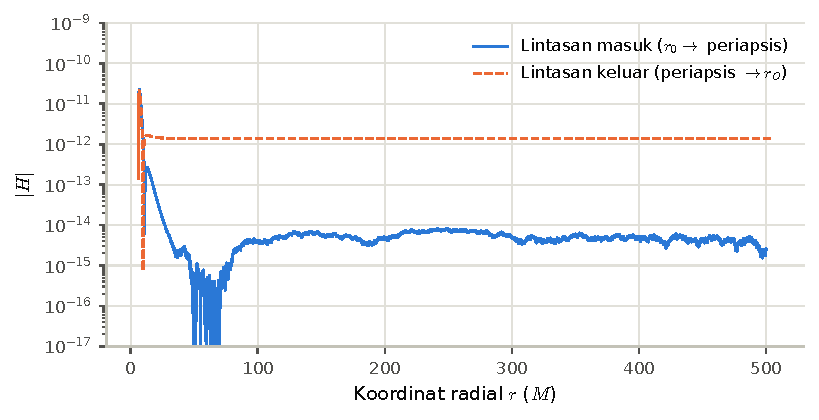
\includegraphics[width=0.85\textwidth]{figures/hamiltonian.pdf}
  \caption{Nilai mutlak Hamiltonian sepanjang lintasan sebagai fungsi koordinat radial, untuk
    $a = 0{,}99$, $\Lambda = 5\times10^{-6}$, dan $b = 7M$, terpisah untuk lintasan masuk dan lintasan keluar.
    Nilai ideal untuk foton adalah $H = 0$.}
  \label{fig:hamiltonian}
\end{figure}

\paragraph{Pembanding eksak.} Untuk seluruh 143 kombinasi $(a, \Lambda)$, sudut defleksi simulasi dan
sudut defleksi eksak dari Pers.~\eqref{eq:orbit} berselisih paling besar $5{,}5\times10^{-7}{}^\circ$. Integrasi
numerik dengan demikian akurat jauh di bawah besar efek $\Lambda$ yang diteliti (orde $10^{-4}$ hingga
$10^{-1}$ derajat). Pembanding eksak juga mengonfirmasi hasil \citet{rindler2007contribution}: di
Schwarzschild--de Sitter, sudut azimut $\phi_{OS}$ bergantung pada $\Lambda$ hanya melalui parameter dampak
efektif $1/b_\text{eff}^2 = 1/b^2 + \Lambda/3$, karena persamaan orbitnya tidak memuat $\Lambda$.

\paragraph{Perbandingan dengan literatur.} Tabel~\ref{tab:validasi} membandingkan hasil untuk
$\Lambda = 0$ dengan nilai \citet{hasanuddin2012pembelokan}, yang menghitung sudut defleksi
\emph{asimtotik} (sumber dan pengamat di tak hingga). Sudut defleksi simulasi pada $r_0 = 500M$ sama dengan
nilai eksak berjarak hingga, dan lebih kecil dari nilai asimtotik eksak hanya sebesar pembelokan yang
terjadi di luar $r_0$ (sekitar $2Mb/r_0^2$ radian, yaitu $0{,}002^\circ$ untuk $b = 5M$ hingga $0{,}018^\circ$
untuk $b = 40M$). Bila offset ruang datar ditambahkan pada nilai koordinat, hasilnya cocok dengan nilai
asimtotik eksak hingga $4{,}5\times10^{-4}{}^\circ$. Nilai \citet{hasanuddin2012pembelokan} sendiri berada
$0{,}08$--$0{,}28^\circ$ di bawah nilai eksak; selisih ini terkonfirmasi oleh deret medan lemah (misalnya
untuk $a = 0{,}52$ dan $b = 40M$, deret memberi $\approx 6{,}10^\circ$). Kolom terakhir menunjukkan bahwa
nilai versi awal $\lvert\phi_{OS} - \pi\rvert$ berbeda dari literatur sebesar offset ruang datar
($1{,}1$--$9{,}1^\circ$). Selisih itu disebabkan definisi, bukan galat numerik; untuk $b = 40M$ nilai
koordinatnya bahkan negatif.

\begin{table}[t]
  \centering
  \small
  \caption{Validasi pada $\Lambda = 0$ terhadap \citet{hasanuddin2012pembelokan}. Semua sudut dalam derajat.
    ``Koord.\ + offset'' adalah $(\phi_{OS} - \pi) + \arcsin(b/r_S) + \arcsin(b/r_O)$; ``Versi awal'' adalah
    $\lvert\phi_{OS} - \pi\rvert$.}
  \label{tab:validasi}
  \begin{tabular}{rrrrrrrr}
    \toprule
    $a$ & $b$ & Hasanuddin & Eksak & $\delta$ & $\delta$ eksak & Koord.\ & Versi \\
        &     & (2012)     & asimtotik & simulasi & $r_0 = 500$ & + offset & awal \\
    \midrule
    \isitabel{tabel/validasi.tex}
    \bottomrule
  \end{tabular}
\end{table}

\FloatBarrier
\subsection{Lintasan foton}

Gambar~\ref{fig:lintasan} menunjukkan lintasan foton di sekitar lubang hitam untuk spin prograde,
Schwarzschild, dan retrograde pada $\Lambda = 0$. Foton retrograde dengan $a = -0{,}99$ melintas sangat dekat
dengan orbit foton kritisnya dan mengitari lubang hitam lebih dari setengah putaran sebelum terhambur,
sehingga sudut defleksinya melebihi $180^\circ$. Lintasan untuk berbagai nilai $\Lambda$ (tidak
ditampilkan) berimpit secara visual. Hal ini sesuai dengan \citet{rindler2007contribution}: bentuk orbit
$r(\phi)$ untuk jarak terdekat tertentu tidak bergantung pada $\Lambda$, dan pengaruh $\Lambda$ muncul
terutama melalui sudut yang diukur di posisi sumber dan pengamat.

\begin{figure}[t]
  \centering
  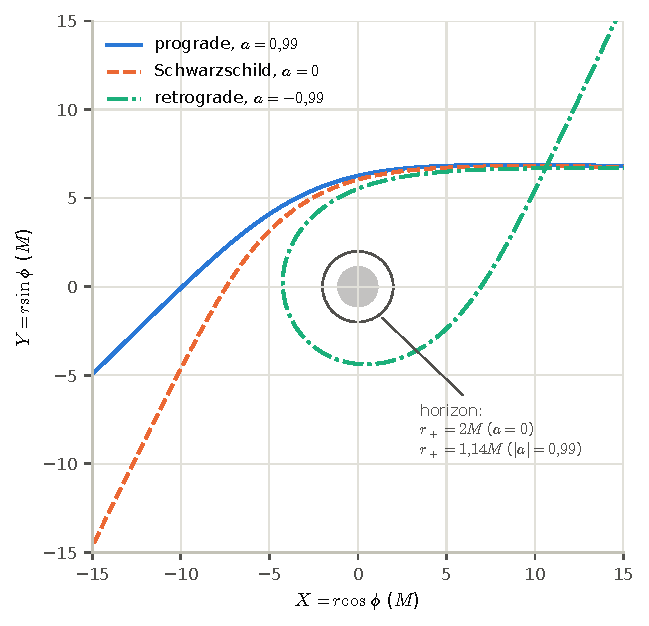
\includegraphics[width=0.62\textwidth]{figures/lintasan.pdf}
  \caption{Lintasan foton dengan $b = 7M$ dan $\Lambda = 0$ di sekitar lubang hitam, untuk spin prograde,
    Schwarzschild, dan retrograde. Foton datang dari kanan ($r_0 = 500M$).}
  \label{fig:lintasan}
\end{figure}

\FloatBarrier
\subsection{Pengaruh spin}

Tabel~\ref{tab:spin} dan Gambar~\ref{fig:spin} menunjukkan sudut defleksi pada $\Lambda = 0$. Spin
prograde memperkecil sudut defleksi, dari $64{,}61^\circ$ ($a = 0$) menjadi $45{,}51^\circ$ ($a = 0{,}99$),
sedangkan spin retrograde memperbesarnya hingga $246{,}06^\circ$ ($a = -0{,}99$). Arah ini sesuai dengan
suku $\mp 4aM/b^2$ pada \citet{jusufi2018gravitational}, \citet{belhaj2022light}, dan
\citet{huang2025influence}, serta dengan hasil eksak \citet{congdon2022asymmetric} bahwa foton retrograde
dibelokkan lebih besar daripada foton prograde.

\citet{congdon2022asymmetric} juga memperingatkan bahwa analogi intuitif seperti ``foton retrograde
melawan arus gravitasi'' dapat menghasilkan kesimpulan yang berlawanan, dan memberikan penjelasan yang
lebih tepat: untuk $|b|$ yang sama, foton retrograde lebih dekat ke parameter dampak kritisnya. Hal ini
terlihat jelas pada Gambar~\ref{fig:spin}(b). Parameter dampak kritis naik dari $5{,}196M$ ($a = 0$) menjadi
$6{,}983M$ ($a = -0{,}99$), sehingga untuk $b = 7M$ foton retrograde ekstrem berada hanya $0{,}017M$ di atas
orbit kritisnya. Untuk $a \to -M$, $b_c \to 7M = b$ dan sudut defleksi divergen
\citep{bozza2002gravitational}.

Kolom terakhir Tabel~\ref{tab:spin} menunjukkan bahwa rumus medan lemah jauh meremehkan sudut defleksi pada
$b = 7M$, terutama untuk spin retrograde. Rumus tersebut hanya berlaku untuk $b \gg b_c$, sehingga
perbandingan dengan artikel pada subbab berikut memakai perubahan akibat $\Lambda$, bukan nilai absolut.

\begin{table}[t]
  \centering
  \small
  \caption{Parameter dampak kritis (Pers.~\ref{eq:bc}) dan sudut defleksi pada $\Lambda = 0$ untuk $b = 7M$.
    Dua kolom terakhir adalah rumus medan lemah, dievaluasi pada jari-jari yang sama.}
  \label{tab:spin}
  \begin{tabular}{rrrrr}
    \toprule
    $a$ & $b_c$ ($M$) & $\delta$ simulasi ($^\circ$) & Huang dkk.\ (24) ($^\circ$) & Belhaj dkk.\ (5.1) ($^\circ$) \\
    \midrule
    \isitabel{tabel/spin.tex}
    \bottomrule
  \end{tabular}
\end{table}

\begin{figure}[t]
  \centering
  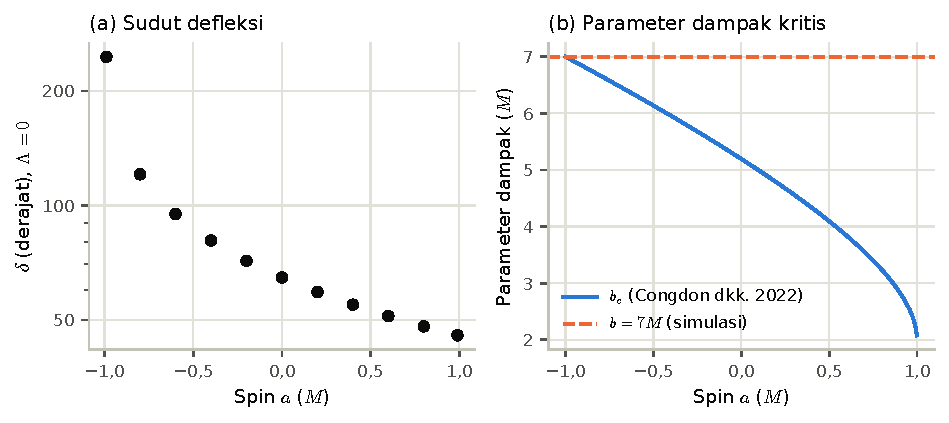
\includegraphics[width=\textwidth]{figures/pengaruh_spin.pdf}
  \caption{(a) Sudut defleksi pada $\Lambda = 0$ terhadap spin (sumbu tegak logaritmik). (b) Parameter
    dampak kritis menurut Pers.~\eqref{eq:bc} dibandingkan dengan parameter dampak simulasi $b = 7M$.}
  \label{fig:spin}
\end{figure}

\FloatBarrier
\subsection{Pengaruh konstanta kosmologi}

Tabel~\ref{tab:grid-positif} dan \ref{tab:grid-negatif} memuat sudut defleksi untuk seluruh kombinasi spin
dan $\Lambda$. Untuk semua spin kecuali $a = -0{,}99$, sudut defleksi \textbf{menurun} secara monoton
terhadap $\Lambda > 0$ dan \textbf{meningkat} terhadap $\Lambda < 0$. Tren ini sesuai dengan
\citet{rindler2007contribution}, yang menyatakan bahwa $\Lambda$ positif ``melawan'' gravitasi; dengan
\citet{belhaj2022light}, yang menemukan bahwa $\Lambda$ negatif menaikkan sudut defleksi dibandingkan
$\Lambda$ positif; dengan \citet{huang2025influence}, yang menyatakan suku $\Lambda$ dan $\Lambda^2$
memperkecil sudut defleksi; serta dengan \citet{pantig2024testing}, yang menemukan sudut defleksi medan
lemah lebih besar untuk $\Lambda$ yang lebih negatif. Besar perubahannya kecil dibandingkan pengaruh spin
(paling besar sekitar $0{,}5^\circ$ pada $\lvert\Lambda\rvert = 5\times10^{-6}$), sehingga perubahan bentuk
lintasan tidak terlihat secara visual.

\begin{table}[t]
  \centering
  \small
  \caption{Sudut defleksi $\delta$ (derajat) untuk $\Lambda \ge 0$ ($M^{-2}$), $b = 7M$.}
  \label{tab:grid-positif}
  \begin{tabular}{rrrrrrrr}
    \toprule
    $a$ & $0$ & $10^{-8}$ & $5\times10^{-8}$ & $10^{-7}$ & $5\times10^{-7}$ & $10^{-6}$ & $5\times10^{-6}$ \\
    \midrule
    \isitabel{tabel/grid_positif.tex}
    \bottomrule
  \end{tabular}
\end{table}

\begin{table}[t]
  \centering
  \small
  \caption{Sudut defleksi $\delta$ (derajat) untuk $\Lambda \le 0$ ($M^{-2}$), $b = 7M$.}
  \label{tab:grid-negatif}
  \begin{tabular}{rrrrrrrr}
    \toprule
    $a$ & $0$ & $-10^{-8}$ & $-5\times10^{-8}$ & $-10^{-7}$ & $-5\times10^{-7}$ & $-10^{-6}$ & $-5\times10^{-6}$ \\
    \midrule
    \isitabel{tabel/grid_negatif.tex}
    \bottomrule
  \end{tabular}
\end{table}

\paragraph{Perbandingan kuantitatif dengan artikel.} Gambar~\ref{fig:pergeseran} membandingkan perubahan
$\delta(\Lambda) - \delta(0)$ hasil simulasi dengan solusi eksak dan dengan rumus
\citet{huang2025influence} dan \citet{belhaj2022light}. Simulasi berimpit dengan solusi eksak. Untuk
$\lvert\Lambda\rvert \le 10^{-6}$ kedua rumus analitik juga cocok dengan simulasi; untuk
$\lvert\Lambda\rvert = 5\times10^{-6}$ keduanya mulai menyimpang karena $\Lambda r_0^2/3 = 0{,}42$, sehingga
ekspansi orde rendah dalam $\Lambda r^2$ tidak lagi akurat. Tabel~\ref{tab:pergeseran} merangkum perubahan
pada $\Lambda = 10^{-6}$: rumus Belhaj dkk.\ berselisih $\le 4{,}1\%$ dan rumus Huang dkk.\ berselisih
$0{,}9\text{--}9{,}2\%$ dari simulasi untuk semua spin kecuali $a = -0{,}99$.

\begin{figure}[t]
  \centering
  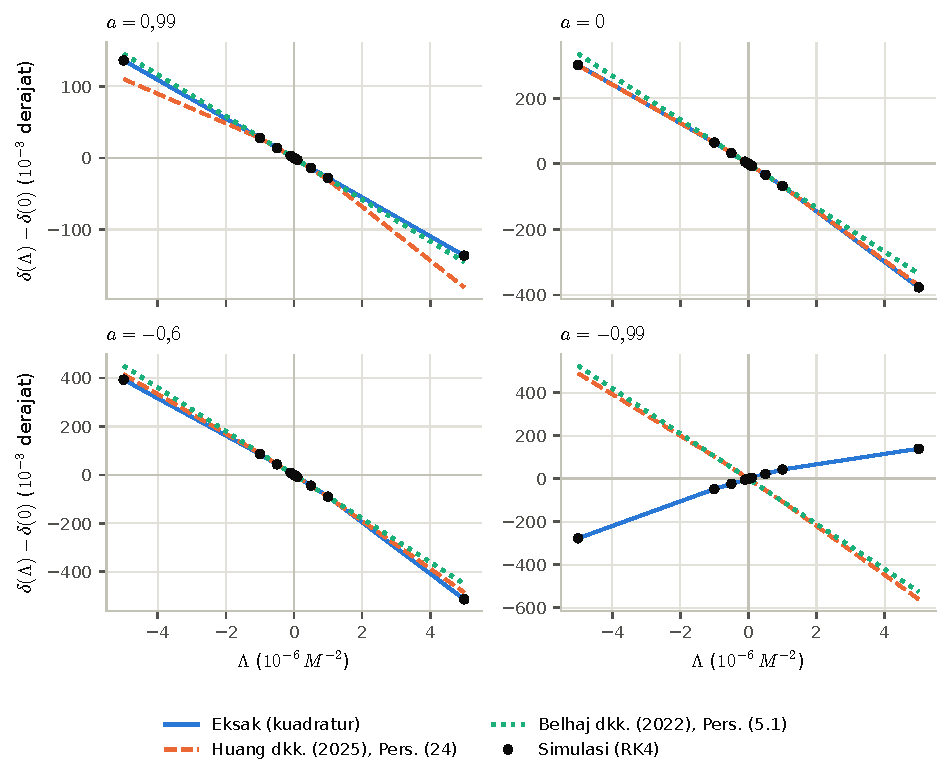
\includegraphics[width=\textwidth]{figures/pergeseran_lambda.pdf}
  \caption{Perubahan sudut defleksi akibat $\Lambda$ untuk empat nilai spin: simulasi (titik), solusi eksak,
    dan rumus analitik \citet[Pers.~24]{huang2025influence} dan \citet[Pers.~5.1]{belhaj2022light}.}
  \label{fig:pergeseran}
\end{figure}

\begin{table}[t]
  \centering
  \small
  \caption{Perubahan sudut defleksi $\delta(\Lambda) - \delta(0)$ pada $\Lambda = 10^{-6}$, dalam
    $10^{-3}$ derajat, beserta selisih relatif rumus analitik terhadap simulasi.}
  \label{tab:pergeseran}
  \begin{tabular}{rrrrrrr}
    \toprule
    $a$ & Simulasi & Eksak & Huang (24) & Selisih (\%) & Belhaj (5.1) & Selisih (\%) \\
    \midrule
    \isitabel{tabel/pergeseran_1e-6.tex}
    \bottomrule
  \end{tabular}
\end{table}

\paragraph{Ketergantungan pada spin.} Gambar~\ref{fig:kemiringan} menunjukkan kemiringan
$\dd\delta/\dd\Lambda$ (dari pencocokan linear untuk $\lvert\Lambda\rvert \le 10^{-6}$) sebagai fungsi spin.
Efek pengurangan oleh $\Lambda$ paling kuat untuk spin retrograde dan melemah untuk spin prograde: kemiringan
berubah dari $(-9{,}21 \pm 0{,}07)\times10^4$ ($a = -0{,}8$) melalui $(-6{,}62 \pm 0{,}04)\times10^4$ ($a = 0$) menjadi $(-2{,}783 \pm 0{,}002)\times10^4$
($a = 0{,}99$), dalam satuan derajat\,$M^2$. Pola ini persis dengan suku $+2a\Lambda(1/u_R + 1/u_S)/3$
pada Pers.~\eqref{eq:belhaj} dan \eqref{eq:huang}: suku $-\Lambda b/(6u)$ tidak bergantung pada spin,
sedangkan suku $a\Lambda$ bernilai positif untuk foton prograde dan negatif untuk foton retrograde.
\citet[\S\,4.1.4]{huang2025influence} juga menyatakan bahwa suku $a\Lambda$ menaikkan sudut defleksi foton
prograde dan menurunkan sudut defleksi foton retrograde. Untuk spin retrograde moderat, nilai mutlak
kemiringan hasil simulasi sedikit lebih kecil daripada rumus analitik (misalnya $4{,}8\%$ untuk
$a = -0{,}8$). Foton tersebut sudah cukup dekat ke orbit kritisnya, sehingga pergeseran $b_c$ yang dibahas
pada Subbab~\ref{subsec:medan-kuat} mulai memberi kontribusi positif.

\begin{figure}[t]
  \centering
  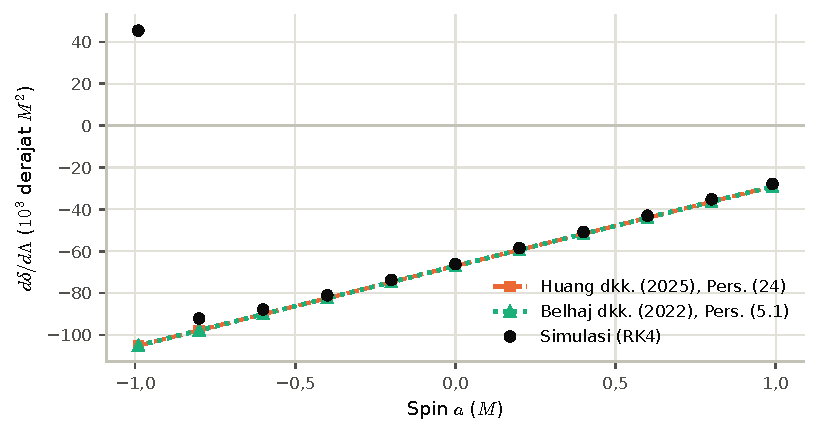
\includegraphics[width=0.88\textwidth]{figures/kemiringan_lambda.pdf}
  \caption{Kemiringan $\dd\delta/\dd\Lambda$ untuk $\lvert\Lambda\rvert \le 10^{-6}$ sebagai fungsi spin:
    simulasi dan rumus analitik. Titik $a = -0{,}99$ berada di rezim medan kuat
    (Subbab~\ref{subsec:medan-kuat}).}
  \label{fig:kemiringan}
\end{figure}

\FloatBarrier
\subsection{Kasus medan kuat: spin retrograde ekstrem}
\label{subsec:medan-kuat}

Untuk $a = -0{,}99$, sudut defleksi justru \emph{meningkat} terhadap $\Lambda > 0$ dan menurun terhadap
$\Lambda < 0$, berlawanan dengan rumus analitik medan lemah (Gambar~\ref{fig:pergeseran}, panel kanan
bawah). Tabel~\ref{tab:medan-kuat} menunjukkan penyebabnya. Foton berada hanya $b - b_c = 0{,}0167M$ di atas
parameter dampak kritis, sehingga sudut defleksinya sangat peka terhadap $b - b_c$:
$\partial\delta/\partial b = -2631^\circ/M$, dibandingkan $-20{,}9^\circ/M$ untuk $a = 0$. Konstanta
kosmologi positif menaikkan $b_c$ (sebesar $2{,}9\times10^{-4}M$ untuk $\Lambda = 5\times10^{-6}$), sehingga
foton bergeser lebih dekat ke orbit kritis. Kontribusi pergeseran ini sekitar $+0{,}76^\circ$, lebih besar
daripada kontribusi suku-suku $\Lambda$ lainnya (sekitar $-0{,}62^\circ$, seorde dengan prediksi
Pers.~\eqref{eq:belhaj}), sehingga totalnya $+0{,}14^\circ$. Ini adalah efek limit medan kuat
\citep{bozza2002gravitational}: dekat orbit kritis, pergeseran kecil $b_c$ menghasilkan perubahan besar
sudut defleksi. Rumus medan lemah \citet{belhaj2022light} dan \citet{huang2025influence} tidak memuat efek
ini, sehingga tidak berlaku untuk kasus tersebut.

\begin{table}[t]
  \centering
  \small
  \caption{Kasus $a = -0{,}99$, $b = 7M$: parameter dampak kritis, jaraknya ke $b$, sudut defleksi, serta
    perubahan sudut defleksi dan nilai koordinat relatif terhadap $\Lambda = 0$ (derajat).}
  \label{tab:medan-kuat}
  \begin{tabular}{rrrrrr}
    \toprule
    $\Lambda$ ($M^{-2}$) & $b_c$ ($M$) & $b - b_c$ ($M$) & $\delta$ & $\Delta\delta$ & $\Delta(\phi_{OS} - \pi)$ \\
    \midrule
    \isitabel{tabel/medan_kuat.tex}
    \bottomrule
  \end{tabular}
\end{table}

\FloatBarrier
\subsection{Perbandingan dengan definisi koordinat (versi awal)}
\label{subsec:dua-definisi}

Versi awal penelitian melaporkan $\lvert\phi_{OS} - \pi\rvert$ dan memperoleh tren yang berlawanan: untuk
$a \ge 0$ nilainya \emph{naik} terhadap $\Lambda > 0$. Tabel~\ref{tab:dua-definisi} dan
Gambar~\ref{fig:dua-definisi} menguraikan sudut defleksi untuk $a = 0{,}99$ menjadi dua bagian,
$\delta = (\phi_{OS} - \pi) + (\Psi_O - \Psi_S + \pi)$. Bagian koordinat naik terhadap $\Lambda$, tetapi bagian
sudut pengamat turun lebih besar, sehingga sudut defleksi totalnya turun.

\begin{table}[t]
  \centering
  \small
  \caption{Dua definisi untuk $a = 0{,}99$. Kolom kedua adalah nilai versi awal (derajat); tiga kolom
    terakhir adalah perubahan relatif terhadap $\Lambda = 0$ dalam $10^{-3}$ derajat.}
  \label{tab:dua-definisi}
  \begin{tabular}{rrrrr}
    \toprule
    $\Lambda$ ($M^{-2}$) & $\lvert\phi_{OS}-\pi\rvert$ & $\Delta(\phi_{OS}-\pi)$ & $\Delta(\Psi_O-\Psi_S+\pi)$ & $\Delta\delta$ \\
    \midrule
    \isitabel{tabel/dua_definisi.tex}
    \bottomrule
  \end{tabular}
\end{table}

\begin{figure}[t]
  \centering
  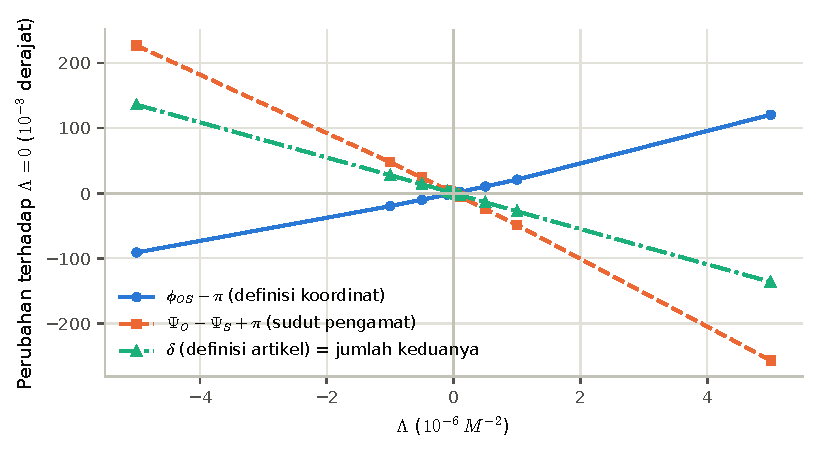
\includegraphics[width=0.88\textwidth]{figures/dua_definisi.pdf}
  \caption{Penguraian perubahan sudut defleksi untuk $a = 0{,}99$ menjadi bagian koordinat dan bagian sudut
    pengamat.}
  \label{fig:dua-definisi}
\end{figure}

Kenaikan bagian koordinat memiliki dua penyebab. Pertama, di Schwarzschild--de Sitter $\Lambda$ hanya mengubah
parameter dampak efektif, $1/b_\text{eff}^2 = 1/b^2 + \Lambda/3$, sehingga untuk $\Lambda > 0$ foton
seolah-olah lewat sedikit lebih dekat dan $\phi_{OS}$ bertambah. Hal ini sesuai dengan suku $\Lambda$ positif
pada $\phi_{OS}$ yang dicatat \citet[\S\,4.1.2]{huang2025influence}. Kedua, untuk lubang hitam berotasi,
koordinat $\phi$ Boyer--Lindquist di Kerr--de Sitter berotasi relatif terhadap kerangka yang tidak berotasi:
kecepatan sudut pengamat ZAMO, $\omega = -g_{t\phi}/g_{\phi\phi}$, mendekati $a\Lambda/3$ pada $r \gg M$.
Selama perjalanan foton (waktu koordinat sekitar $10^3M$), $\phi$ bertambah sekitar $(a\Lambda/3)\,\Delta t$,
yaitu $+0{,}116^\circ$ untuk $a = 0{,}99$ dan $\Lambda = 5\times10^{-6}$. Suku ini ikut tanda $a$, sehingga
pada versi awal sudut koordinat untuk spin retrograde moderat justru turun terhadap $\Lambda$.

Sebaliknya, sudut yang diukur pengamat statis mengecil kuat untuk $\Lambda > 0$, karena faktor
$\sqrt{1 - 2M/r - \Lambda r^2/3}$ pada $\sin\psi$ turun dari $0{,}998$ menjadi $0{,}761$ pada $r = 500M$ dan
$\Lambda = 5\times10^{-6}$. Inilah suku $-\Lambda b/(6u)$ pada Pers.~\eqref{eq:belhaj} dan
\eqref{eq:huang}, yang sejalan dengan pernyataan \citet{rindler2007contribution} bahwa kontribusi $\Lambda$
berasal dari metrik, bukan dari persamaan orbit. Pengecilan sudut yang diukur pengamat statis juga sejalan
dengan hasil \citet{afrin2022estimating} bahwa $\Lambda$ memperkecil ukuran bayangan lubang hitam yang
dilihat pengamat statis.

Jadi, angka-angka versi awal benar sebagai sudut koordinat, tetapi besaran tersebut bukan sudut yang
diukur pengamat dan tidak dapat dibandingkan langsung dengan artikel acuan. Kesimpulan bahwa ``$\Lambda$
positif meningkatkan sudut defleksi'' hanya berlaku untuk sudut koordinat tersebut.

\FloatBarrier
\subsection{Hasil pencocokan kurva}

Untuk $a = 0{,}99$ (Gambar~\ref{fig:fitting}a), pencocokan model pangkat memberi
\begin{align}
  \Lambda > 0:&\quad \delta = (-23\,251 \pm 412)\,\Lambda^{0{,}9869 \pm 0{,}0015} + 45{,}5090, \\
  \Lambda < 0:&\quad \delta = (23\,442 \pm 294)\,\lvert\Lambda\rvert^{0{,}9878 \pm 0{,}0010} + 45{,}5090,
\end{align}
dengan $R^2 > 0{,}99999$. Koefisien $A$ negatif untuk $\Lambda > 0$ menegaskan bahwa sudut defleksi menurun.
Eksponen $B$ sedikit di bawah 1, tetapi penyimpangan ini tidak mencerminkan kopling fisis antara lubang hitam
dan latar de Sitter. Penyimpangan tersebut berasal dari suku orde tinggi dalam $\Lambda r_0^2$, karena sumber
berada di $r_0 \approx 0{,}65\,r_c$ untuk $\Lambda = 5\times10^{-6}$. Bila sumber dan pengamat
dipindahkan ke $r_0 = 100M$, pencocokan yang sama pada solusi eksak memberi $B = 1{,}00010 \pm 0{,}00003$, dibandingkan
$B = 0{,}9869 \pm 0{,}0015$ pada $r_0 = 500M$. Untuk $\lvert\Lambda\rvert \le 10^{-6}$ hubungannya praktis linear, dengan
kemiringan $(-2{,}783 \pm 0{,}002)\times10^4$\,derajat\,$M^2$. Nilai $R^2 \approx 1$ pada tujuh titik monoton dengan tiga
parameter tidak dengan sendirinya membuktikan suatu hukum fisis.

\begin{figure}[t]
  \centering
  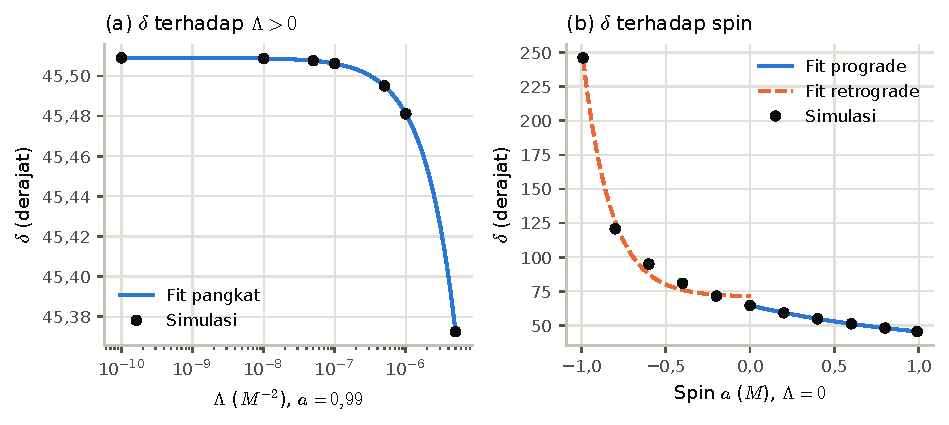
\includegraphics[width=\textwidth]{figures/fitting.pdf}
  \caption{(a) Sudut defleksi terhadap $\Lambda > 0$ untuk $a = 0{,}99$ dengan model pangkat. (b) Sudut
    defleksi terhadap spin pada $\Lambda = 0$ dengan model eksponensial terpisah untuk spin prograde dan
    retrograde.}
  \label{fig:fitting}
\end{figure}

Untuk ketergantungan pada spin pada $\Lambda = 0$ (Gambar~\ref{fig:fitting}b), model eksponensial cocok
dengan baik untuk spin prograde,
$\delta = (32{,}4 \pm 0{,}6)\,e^{-(0{,}894 \pm 0{,}028)\,a} + (32{,}2 \pm 0{,}7)$ ($R^2 = 0{,}99996$), tetapi kurang cocok untuk spin retrograde,
$\delta = (0{,}44 \pm 0{,}35)\,e^{-(6{,}0 \pm 0{,}8)\,a} + (71 \pm 5)$ ($R^2 = 0{,}9931$). Model eksponensial hanya bersifat deskriptif: untuk foton
retrograde, $b_c \to 7M$ ketika $a \to -M$, sehingga untuk $b = 7M$ sudut defleksi divergen secara logaritmik
\citep{bozza2002gravitational,congdon2022asymmetric}, dan kurva tersebut tidak boleh diekstrapolasi ke
$a = -1$.

\FloatBarrier
\subsection{Signifikansi fisis dan keterbatasan}

Nilai $\Lambda$ yang disimulasikan sangat besar dibandingkan nilai kosmologis. Konstanta kosmologi hasil
pengamatan sekitar $1{,}1\times10^{-52}\,\text{m}^{-2}$; untuk lubang hitam Sgr A* ($M \approx 4\times10^6$
massa Matahari, $GM/c^2 \approx 6\times10^9$\,m), nilai ini setara dengan $\Lambda \sim 4\times10^{-33}M^{-2}$,
sekitar $10^{24}$--$10^{27}$ kali lebih kecil dari nilai simulasi. Karena efek utamanya sebanding dengan
$\Lambda b\,r$, nilai $\Lambda$ yang besar pada simulasi ini dapat dipandang sebagai cara memperbesar efek
yang secara fisis hanya berarti bila sumber dan pengamat sangat jauh. \citet{rindler2007contribution}
menaksir bahwa untuk sinar yang menyinggung Matahari kontribusi $\Lambda$ sekitar $10^{28}$ kali lebih kecil
daripada pembelokan Einstein, sedangkan \citet{huang2025influence} memperkirakan bahwa koreksi suku-suku
barunya dapat mencapai orde $10\,\mu$as untuk bintang-bintang di dekat Sgr A*.

Keterbatasan penelitian ini adalah sebagai berikut.
\begin{enumerate}
  \item Hanya orbit di bidang ekuator ($\theta = \pi/2$) yang ditinjau.
  \item Sumber dan pengamat berada pada jarak hingga ($r_0 = 500M$, $r_O \approx 505M$). Definisi
        sudut defleksi untuk ruang-waktu yang tidak datar asimtotik belum seragam dalam literatur
        \citep{arakida2018light,hu2022light}; penelitian ini mengikuti definisi
        \citet{ishihara2016gravitational} yang dipakai \citet{belhaj2022light} dan \citet{huang2025influence}.
  \item Rumus analitik pembanding adalah ekspansi medan lemah, sehingga hanya perubahan akibat $\Lambda$ yang
        dapat dibandingkan pada $b = 7M$.
  \item Integrasi memakai langkah tetap tanpa kontrol galat adaptif; galat membesar untuk $b$ yang sangat
        dekat dengan $b_c$ (misalnya $\max|H| \approx 2\times10^{-10}$ untuk $a = 0$, $b = 5{,}2M$).
  \item Kriteria tangkapan memakai horizon Kerr ($\Lambda = 0$); perbedaannya dengan horizon
        Kerr--de Sitter kurang dari $2\times10^{-5}M$ dan hanya memengaruhi foton yang tertangkap.
\end{enumerate}

% =====================================================================================
\section{Kesimpulan dan Saran}

\subsection{Kesimpulan}

\begin{enumerate}
  \item Persamaan gerak foton di ruang-waktu Kerr--de Sitter berhasil diturunkan dari Hamiltonian secara
        simbolik dan diselesaikan dengan RK4. Konservasi Hamiltonian terjaga ($|H| \lesssim 5\times10^{-11}$)
        dan sudut defleksi simulasi sesuai dengan solusi eksak hingga $5{,}5\times10^{-7}{}^\circ$.
  \item Spin prograde memperkecil dan spin retrograde memperbesar sudut defleksi, sesuai dengan
        \citet{congdon2022asymmetric} dan suku $\mp 4aM/b^2$ pada rumus analitik. Pada $b = 7M$, sudut
        defleksi berkisar dari $45{,}5^\circ$ ($a = 0{,}99$) hingga $246{,}1^\circ$ ($a = -0{,}99$).
  \item Dengan definisi sudut defleksi pada jarak hingga yang dipakai artikel acuan, konstanta kosmologi
        positif \emph{memperkecil} sudut defleksi dan konstanta kosmologi negatif memperbesarnya, sesuai
        dengan \citet{rindler2007contribution}, \citet{belhaj2022light}, \citet{huang2025influence}, dan
        \citet{pantig2024testing}. Pada $\Lambda = 10^{-6}$, rumus Belhaj dkk.\ dan Huang dkk.\ cocok dengan
        simulasi dengan selisih di bawah $10\%$.
  \item Efek pengurangan oleh $\Lambda$ melemah untuk spin prograde dan menguat untuk spin retrograde, sesuai
        dengan suku $a\Lambda$ pada rumus analitik.
  \item Pada spin retrograde ekstrem ($a = -0{,}99$), foton berada sangat dekat dengan orbit kritisnya;
        pergeseran parameter dampak kritis oleh $\Lambda$ membalik tren tersebut, sesuai dengan limit medan
        kuat \citet{bozza2002gravitational}.
  \item Sudut koordinat $\lvert\phi_{OS} - \pi\rvert$ yang dipakai pada versi awal penelitian memberi tren
        $\Lambda$ yang berlawanan karena tidak memuat sudut yang diukur pengamat dan memuat efek rotasi
        koordinat Boyer--Lindquist. Besaran tersebut tidak dapat dibandingkan langsung dengan artikel acuan.
\end{enumerate}

\subsection{Saran}

\begin{enumerate}
  \item Memperluas variasi parameter dampak $b$, dari medan lemah hingga mendekati $b_c$, untuk memetakan
        transisi dari rezim rumus medan lemah ke rezim medan kuat.
  \item Menghitung koefisien limit medan kuat $\bar a$ dan $\bar b$ \citep{bozza2002gravitational} untuk
        Kerr--de Sitter dan membandingkannya dengan kasus $a = -0{,}99$.
  \item Meninjau orbit di luar bidang ekuator dan definisi sudut defleksi alternatif, misalnya relatif
        terhadap latar de Sitter \citep{arakida2018light}.
  \item Menggunakan integrator dengan langkah adaptif untuk parameter dampak yang sangat dekat dengan $b_c$.
\end{enumerate}

% =====================================================================================
\bibliographystyle{plainnat}
\bibliography{daftar_pustaka}

\appendix
\section{Reproduksi hasil}

Seluruh kode berada di repositori penelitian (paket \texttt{kerr\_ds}). Data, gambar, dan tabel laporan ini
dibuat ulang dengan
\begin{verbatim}
python docs/laporan_akhir/generate_results.py
\end{verbatim}
yang menjalankan 153 simulasi (sekitar 15 menit pada CPU 4 inti) dan menyimpan hasilnya di
\texttt{docs/laporan\_akhir/data/} (\texttt{hasil\_grid.csv}, \texttt{validasi.csv}, \texttt{ringkasan.json}).
Notebook \texttt{Lambda\_Deflection.ipynb}, \texttt{Spin\_Deflection.ipynb}, dan \texttt{Validation.ipynb}
menampilkan analisis yang sama secara interaktif, dan \texttt{pytest} menjalankan uji regresi serta uji
terhadap solusi eksak dan rumus analitik. Penjelasan metode yang lengkap ada di \texttt{docs/METHODOLOGY.md}.

\end{document}
